\subsection{Flujo de efectivo}

A través del flujo de efectivo es posible determinar que capacidad tiene la empresas para generar efectivo de manera que cumpla con sus compromisos, inversiones y demás procesos de expansión. 

Existen 3 tipos de flujos de caja para tener el flujo neto:

\begin{itemize}
    \item \textbf{Flujo de caja de operación: } Tomando la utilidad producto del estado de resultados, depreciación, amortización, intereses de la deuda y los impuestos a la rente.
    \item \textbf{Flujo de caja de inversión: } Se engloba toda la inversión realizada para hacer funcionar la empresa, tomando en cuenta las inversiones tangibles e intangibles.
    \item \textbf{Flujo de caja de financiamiento: } Utiliza el dinero que llega por medio de inversionistas y sus pagos.
\end{itemize}

La suma general de estos 3 tipos da como resultado la cantidad que la empresa genero en el año analizado.

\vspace{2mm}
\begin{minipage}{0.8\textwidth}
\centering
\captionof{table}[{Flujo de caja de operación }]{ Flujo de caja de operación}
\label{flujoOperacional}
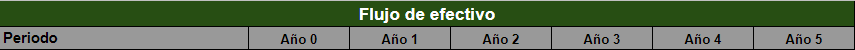
\includegraphics[width=1.2\textwidth]{Images/tiempo.png}
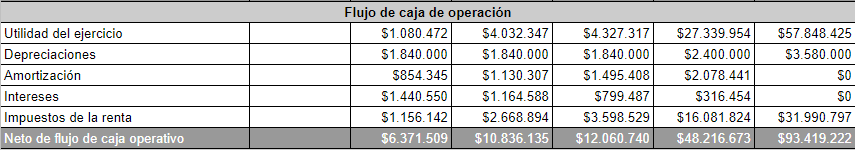
\includegraphics[width=1.2\textwidth]{Images/flujoEfectivoOperacion.png}
\fnote{Nota. \textup{Fuente : Autores}}
\end{minipage}

\vspace{2mm}
\begin{minipage}{0.8\textwidth}
\centering
\captionof{table}[{Flujo de caja de inversión }]{ Flujo de caja de inversión }
\label{flujoInversion}
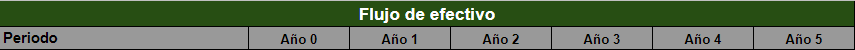
\includegraphics[width=1.2\textwidth]{Images/tiempo.png}
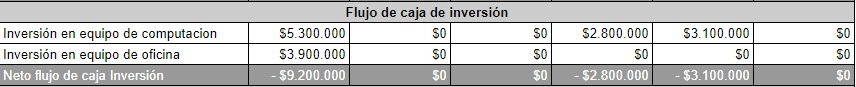
\includegraphics[width=1.2\textwidth]{Images/flujoEfectivoInversion.png}
\fnote{Nota. \textup{Fuente : Autores}}
\end{minipage}

\vspace{2mm}
\begin{minipage}{0.8\textwidth}
\centering
\captionof{table}[{Flujo de caja de financiamiento }]{ Flujo de caja de financiamiento }
\label{flujoFinanciamiento}
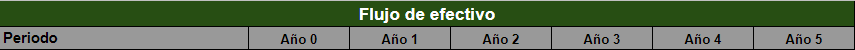
\includegraphics[width=1.2\textwidth]{Images/tiempo.png}
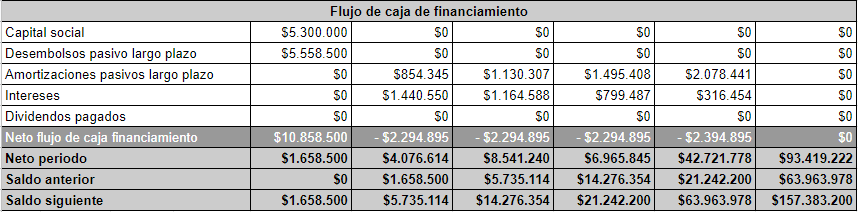
\includegraphics[width=1.2\textwidth]{Images/flujoEfectivoFinanciamiento.png}
\fnote{Nota. \textup{Fuente : Autores}}
\end{minipage}
